%********************************NO TITLE/CONTENTS PAGE TEMPLATE*****************************

%******************* Packages ***************************************************************
\documentclass[11pt]{article}
\usepackage[margin = 2.5cm, includefoot]{geometry}
\usepackage{amsfonts, amsmath, amssymb} 		%math packages
\usepackage[none]{hyphenat}						%prevent hyphenated words, why??
\usepackage{fancyhdr}							%headers and footers
\usepackage{graphicx}							%table package?
\usepackage{float}								%image package?
\usepackage[nottoc, notlot, notlof]{tocbibind}	%contents packages?
\usepackage{fixltx2e}							%\textsubscript{} and \textsuperscript{}
\usepackage{xcolor}								%font colors \color{red} \color{black} etc.
\usepackage{url}								%ignores all special characters contained \url{URL} 
%can use \usepackage{hyperref} for clickable url \url{URL}
\usepackage{amsmath, amssymb, cancel, units}	%math styles (\dfrac{num}{den})
\usepackage{titlesec}							%title spacing options
\usepackage{siunitx}							%scientific notation package
\usepackage{tikz}								%drawing package (\begin{tikzpicture \end{tikzpicture})
\usepackage{physics}							%for absolute value symbol \abs
\usepackage{verbatim}							%for comment blocks (\begin{comment})
\usepackage{subcaption}							%subfigures \begin{subfigure}{width}
\usetikzlibrary{calc}
\usepackage{multicol}

%******************** Preamble - i.e. formatting for whole page ***************
%\pagestyle{fancy}								%use fancy style
\fancyhead{}									%clear header and footer
\fancyfoot{}
%\fancyhead[L]{\slshape\MakeUppercase{LeftHeader}}	%italics and uppercase
%\fancyhead[R]{RightHeader}
\fancyfoot[C]{\thepage}								%page number
\renewcommand{\headrulewidth}{0.5pt}				%set header line width to _pt
\renewcommand{\footrulewidth}{0.5pt}				%set footer line width to _pt

\parindent 0ex									%remove paragraph indents
%\setlength{\parindent}{4em}					%adjust indent legnth if wanted
\setlength{\parskip}{1em}						%adjust spacing between paragraphs
\renewcommand{\baselinestretch}{1}				%line spacing of paragraphs

\newcommand\tab[1][1cm]{\hspace*{#1}}			%custom tab command
\newcommand{\ddt}[1]{\dfrac{d#1}{dt}}			%custom d/dt command
\newcommand{\degrees}{^\circ}
% !TeX spellcheck = en_GB 
	
	\begin{document}
		
		%****************** Body ********************
		\title{\vspace{-2.5cm}ZEIT4230 Engineering Design Practise (z3419283 - Alex Gee)\\
			Obstacle Detection System - Theoretical Overview:}
		\date{}
		\author{}
		\maketitle
		\vspace{-1.5cm}
			
		\section{Hardware}
			\subsection{HC-SR04 Ultrasonic Sensors}
					The HC-SR04 is the main (internal to system) hardware that the ODS will utilise. It has an ultrasonic transmitter and receiver module to measure the distance to an object within its range (2-400cm) \cite{hcsr04Manual}. Ultrasonic sensors send out an ultrasonic sound wave pulse, measuring the time taken to detect a reflection and using the known speed of sound to calculate the distance to an object. The HC-SR04 specifically transmits an 8-cycle burst at 40kHz as shown in Figure \ref{fig:hcsr04Pulses} and returns a pulse width equal to the time taken for a reflection to be detected. 
					
					\begin{figure}[H]
						\centering
						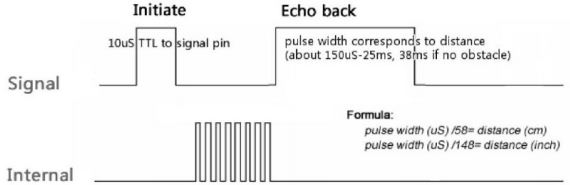
\includegraphics[width=0.6\linewidth]{Images/hcsr04Pulses.jpg}
						\caption{Operation Signals \cite{hcsr04Manual}}
						\label{fig:hcsr04Pulses}
					\end{figure}
										
					This reflection time is the time taken for the signal to travel from the transmitter, to the object and back again, and hence for one way distance $d$ it must be divided by 2 as shown in equation \ref{eq:distance}.
					%
					\begin{equation}\label{eq:distance}
						d = \frac{ct}{2}
					\end{equation}
					%
					Where $c$ is speed of sound and $t$ is the pulse width.
					
					Since sound tends to travel outward from the source in all directions, getting a narrow beam is inherently difficult. The expected angular performance of the sensor is shown below in Figure \ref{fig:hcsr04Performance}.
					
					\begin{figure}[H]
						\centering
						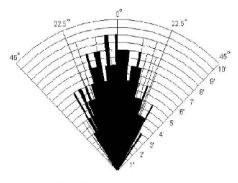
\includegraphics[width = 0.4\linewidth]{Images/hcsr04Performance.jpg}
						\caption{HC-SR04 Performance Results \cite{hcsr04Manual}}
						\label{fig:hcsr04Performance}
					\end{figure}
				
					The beamwidth $\approx \pm 30\degrees$, with a range of up to 400cm (i.e. 8x50cm grid squares), hence the sensor will pick up obstacles left and right of its front but it will be difficult to distinguish which box it is in. As an example some basic trigonometry shown in equation \ref{eq:xBoxes}, shows $\approx$ 3 grids to the left and right of the forward box at the 300cm mark will be picked up:
					%
					\begin{align}\label{eq:xBoxes}
						\tan(30\degrees) 	& = \dfrac{300cm}{x}\nonumber\\
						\implies x			& = 300\tan(30\degrees)\nonumber\\
								 			& = 173.2cm\nonumber\\
											& \approx 3.5 \text{ grid squares}
					\end{align}
					%
					This is shown in Figure \ref{fig:beamwidth}
					\begin{figure}[H]
						\begin{center}
							\begin{tikzpicture}[scale = 0.015]

							\draw (0,0) -- (0,300);
							\draw(0,300) -- (173.2,300);
							\draw(0,0) -- (173.2,300);
							\draw(0,0) -- (-173.2,300);
							\draw(0,300) -- (-173.2,300);
							\draw (-25,300) rectangle (25,350);
							\draw (25,300) rectangle (75,350);
							\draw (75,300) rectangle (125,350);
							\draw (125,300) rectangle (175,350);
							
							\draw (-15,200) node[left,rotate=90]{300cm};
							\draw(10,100) node[right]{$30\degrees$};
							\draw(-3,100) node[left]{$30\degrees$};

							\end{tikzpicture}
							\caption{HC-SR04 Beamwidth}
							\label{fig:beamwidth}
						\end{center}
					\end{figure}
				
				\subsection{TMP36 Temperature Sensor}
					Based on the temperature dependence of the speed of sound (see Section \ref{section:sound}) a temperature sensor may be required. A comparison of the various sensors found at core electronics can be seen below in Table \ref{tab:tempSensors}.
					
					%
					\begin{table}[H]													
						\centering														
						\begin{tabular}{|c|c|c|c|c|c|}\hline
							\textbf{Sensor}	& \textbf{Accuracy ($\degrees C$)} 	& \textbf{$\approx$ Error at 400cm} 	& \textbf{Cost}		& \textbf{Notes}			\\ \hline
							DHT22 			& $\pm 0.5$							& $\pm 0.35$							& \$13.18			& Temperature and humidity	\\ \hline
							DHT11 			& $\pm 2$							& $\pm 1.41$ 							& \$5.80			& Temperature and humidity	\\ \hline
							TMP36 			& $\pm 2$							& $\pm 1.41$ 							& \$2.18			& 							\\ \hline
							LM35DZ 			& $\pm 0.4$							& $\pm 0.28$							& \$3.40			& Supply Voltage: 4V - 30V	\\ \hline
						\end{tabular}
						\caption{Temperature Sensor Options \cite{dht11Datsheet}, \cite{dht22Datsheet}, \cite{lm35dzDatasheet}, \cite{tmp36Datasheet}, \cite{tempSensorPrices}}		% table caption
						\label{tab:tempSensors}			%Table number
					\end{table}
					%
					The error has been calculated by combining equations \ref{eq:distance} and \ref{eq:soundSpeed}, with a known distance of 400cm as shown below:
					
					\begin{align}
						error 			& = d_{actual} - d_{measured}	\tab \text{Where: }\\
						d_{measured} 	& = \dfrac{c_{measured}t}{2} \nonumber\\
						t 				& = \dfrac{2d}{c_{actual}}	\nonumber\\
						c_{measured} 	& = 331.4 + 0.6\times(T+T_{error}) 	\nonumber
					\end{align}
					\textit{Note: t = duration, $d_{actual} = 400cm$, $d_{measured}$ = calculated distance from error temperature, $c_{measured}$ = calculated speed of sound based on error temperature, $c_{actual}$ = known speed of sound at $20\degrees C$}
					
			\section{Speed of Sound}\label{section:sound}
				The speed of sound changes based on the medium it is travelling through. For the purpose of this project the effect of temperature will be the main consideration and its effect can be found according to equation \ref{eq:soundSpeed} below:
				%
				\begin{equation}\label{eq:soundSpeed}
					c = 331.5 + 0.6T
				\end{equation}
				%
				\cite{soundTemp} At $20\degrees C$, $c = 343m/s$ which can be used as a good estimate in simple circumstances, however if a higher degree of accuracy is required, temperature will need to be considered.
				
			\section{Trigonometry}
				To make the calculations of where the obstacle is relative to the sensors and in turn relative to the Location System device (POZYX), the following trigonometric functions must be understood:
				\begin{multicols}{2}
					\begin{figure}[H]
						\begin{center}
							\begin{tikzpicture}[scale = 0.015]
							
							\draw (0,0) -- (0,300);
							\draw(0,300) -- (173.2,300);
							\draw(0,0) -- (173.2,300);
							
							\draw (-15,200) node[left,rotate=90]{adj};
							\draw(0,50) node[right]{$\theta$};
							\draw(75,300) node[above]{opp};
							\draw(80,150) node[below, rotate = 60]{hyp};
							
							\end{tikzpicture}
							\caption{Right Angled Triangle}
							\label{fig:trig}
						\end{center}
					\end{figure}
				
					\begin{align}
						\sin(\theta) 	& = \dfrac{opp}{hyp}	\nonumber\\
						\cos(\theta) 	& = \dfrac{adj}{hyp}	\nonumber\\
						\tan(\theta) 	& = \dfrac{opp}{adj}	\nonumber\\
						hyp^2 			& = opp^2 + adj^2
					\end{align}
				\end{multicols}
					
					
		\newpage
			\begin{thebibliography}{}
				\bibitem{hcsr04Manual}
				Cytron Technologies Sdn. Bhd., 2013, Cytron Technologies, accessed 19 March 2018, \url{<http://web.eece.maine.edu/~zhu/book/lab/HC-SR04%20User%20Manual.pdf>}
					
				\bibitem{ultrasonicFreqs}
				BBC 2013, BBC, accessed 19 March 2018, \url{<URL of site>}
				
				\bibitem{soundTemp}
				Wong, C 2000, hypertextbook, accessed 20 March 2018, \url{<https://hypertextbook.com/facts/2000/CheukWong.shtml>}
				
				\bibitem{dht22Datsheet}
				Liu, T Core Electronics, accessed 20 March 2018, \url{<https://core-electronics.com.au/attachments/DHT22.pdf>}
				
				\bibitem{dht11Datsheet}
				Aosong Electronics, accessed 20 March 2018, \url{<https://akizukidenshi.com/download/ds/aosong/DHT11.pdf>}
				
				\bibitem{lm35dzDatasheet}
				National Semiconductor, accessed 20 March 2018, \url{<http://www.futurlec.com/Linear/LM35DZ.shtml>}
				
				\bibitem{tmp36Datasheet}
				Analog Devices, Core Electronics accessed 20 March 2018, \url{<http://dlnmh9ip6v2uc.cloudfront.net/datasheets/Sensors/Temp/TMP35_36_37.pdf>}
				
				\bibitem{tempSensorPrices}
				Core Electronics, accessed 20 March 2018, \url{<https://core-electronics.com.au/search/?fq%5Bcategory%5D=Temperature+%26+Humidity&fq%5Bcategory_id%5D=892&q=%2A%2A>}
				
				%to cite: \cite{ref1}
				
				
				
				% ***** Different Reference Type formats *********
				%\bibitem{Book1}
				%Surname, Initial. Surname, Initial. Year \textit{Book name with minimal capitalisation}, 1st edn, Publisher, Place of Publication
				
				%to cite: \cite{Book1}
				
				%\bibitem{Website1}
				%author (person/organisation) YEAR (creation/update), Site Sponsor, accessed 1 January 1999, \url{<URL of site>}
				
				%to cite: \cite{Website1}
				
			\end{thebibliography}
			
		
	\end{document}

%******************* Useful quick formatting ************************
%																	*
				%********* Table Example ************					*
%\begin{table}[H]													
%	\centering														
%	\begin{tabular}{|c|c|c|c|c|c|}\hline
%		$x$ & 0 & 1 & 2 & l & r\\ \hline
%		$f(x)$ & 3 & 6 & 9 & l & r\\ \hline
%		
%	\end{tabular}
%	\caption{Table caption}		% table caption
%	\label{tab:data1}			%Table number
%\end{table}

%\ref{tab:data1}			%to reference

			%********** Figure example *************
%\begin{figure}[H]
%	\centering
%	\includegraphics[scale=0.5]{sample_image.JPG}
%	\caption{Image Caption}
%	\label{fig:imag1}
%\end{figure}

%\ref{fig:imag1}			%to reference

			%********* Subfigure example **********
\begin{comment}
\begin{figure}[H]
	\centering
	\begin{subfigure}{.5\textwidth}
		\centering
		\includegraphics[width=\linewidth]{image1.jpg}
		\caption{Subimage a}
		\label{fig:image1}
	\end{subfigure}%
	\begin{subfigure}{.5\textwidth}
		\centering
		\includegraphics[width=\linewidth]{image2.jpg}
		\caption{Subimage b}
		\label{fig:image2}
	\end{subfigure}
	\caption{Whole Figure caption}
	\label{fig:wholeFigureLabel}
\end{figure}
\end{comment}



			%*********** Lists *******************
%Bullet points
%\begin{itemize}
%	\item Entry 1
%	\item Entry 2...
%\end{itemize}

%Ordered list
%\begin{enumerate}
%	\item Item 1
%	\item Item 2
%\end{enumerate}

%Nested ordered list
%\begin{enumerate}
%	\item first level 1
%	\item first level 2
%	\begin{enumerate}
%		\item second level a
%		\item second level b
%		\begin{enumerate}
%			\item third level i
%			\item third level ii
%			\begin{enumerate}
%				\item fourth level A
%				\item fourth level B
%			\end{enumerate}
%			\item third level iii
%		\end{enumerate}
%		\item second level c
%	\end{enumerate}
%	\item first level 3
%\end{enumerate}

%************* Equations ********************
% can use $equation$ for in text equation
% or $$equation$$ for new line equation
% or for numbered/referenced equations:

%\begin{equation} \label{eq:reference}			
%	equation
%\end{equation}

% reference using \eqref{reference} for brackets, or \ref{reference} for no brackets

%************ DRAWING WITH TIKZPICTURE EXAMPLE ***********************
\begin{comment}
\begin{figure}[H]
	\begin{center}
		\begin{tikzpicture}[scale = 0.9]
		\draw (0,0) rectangle (7,10);
		\draw (0,10) -- (7,8);
		\draw (7,8) -- (0,6);
		\draw (0,6) -- (7,4);
		\draw (7,4) -- (0,2);
		\draw (0,2) -- (7,0);
		\draw (0.5,0) -- (0.5,10);
		\draw (6.5,0) -- (6.5,10);
		\draw (0.5,10) node[above]{$V_{in}$};
		\draw (6.5,10) node[above]{$V_L$};
		\draw (0,10) node[left]{$t_0$};
		\draw (0,6) node[left]{$t_2$};
		\draw (0,2) node[left]{$t_4$};
		\draw (7,8) node[right]{$t_1$};
		\draw (7,4) node[right]{$t_3$};
		\draw (7,0) node[right]{$t_5$};		
		\draw (3.5,10) node[above]{$l$};
		\draw (3.5,9) node[above]{$V_0^+$};
		\draw (3.5,7.1) node[above]{$V_0^+ + V_0^-$};
		\draw (3.5,5.3) node[above]{$V_0^+ + V_0^- + V_1^+$};
		\draw (3.5,3.4) node[above]{$V_0^+ + V_0^- + V_1^+ + V_1^-$};
		\draw (3.5,1.5) node[above]{$V_0^+ + V_0^- + V_1^+ + V_1^- + V_2^+$};
		\end{tikzpicture}
		\caption{Bounce Diagram}
		\label{fig:bounce}
	\end{center}
\end{figure}
\end{comment}





















